\documentclass[a4paper, 11pt]{article}

% Packages
\usepackage[a4paper, inner=2.5cm, outer=2.5cm, top=2.5cm, bottom=2.5cm, bindingoffset=0cm]{geometry}
\usepackage{amsmath,amsthm,amssymb,amsfonts}
\usepackage{graphicx}
\usepackage[colorlinks=true, allcolors=blue]{hyperref}
\usepackage{fontspec,xunicode,xltxtra}
\usepackage{biblatex}
\usepackage{csquotes}
\usepackage{svg}

% GERMAN
\usepackage[ngerman=ngerman-x-latest]{hyphsubst}
\usepackage[ngerman]{babel}

% ENGLISH
%\usepackage[USenglish]{babel}
%\usepackage{hyphsubst}

% Figures
\graphicspath{{figures/}}

% Citations
\addbibresource{bib/main.bib}

\begin{document}

\title{\vspace{-2.0cm}CT Präsentationsprüfung\\Zusammenfassung}
\author{Marvin Borner}
\date{\today}

\maketitle

%\tableofcontents

\section{Präsentation}
\subsection{Grober Aufbau}

\begin{enumerate}
	\item Deckblatt
	\item Inhalt (Gliederung - Beschreiben)
	\item Problemstellung
	\item Grundlagen
	\item Hauptteil
	\item Schluss/Fazit
	\item IDE/Demonstration
\end{enumerate}

\subsection{Hinweise}
\begin{itemize}
	\item Keine dunkle IDE nutzen (sieht man nicht gut auf dem Beamer - 2NP Abzug!)
	\item Nicht monoton reden (=> Motiviert sein!)
	\item max. 12min Vortrag; 8min Kolloquium/Fragen
\end{itemize}

\section{Kolloquium Themen}

\subsection{Patterns (Entwurfsmuster)}
Muster für wiederkehrende Entwurfsprobleme in der Softwarearchitektur und -entwicklung => Vorlagen zur Problemlösung.

Relevante Muster:
\begin{itemize}
	\item \textbf{Drei-Schichten-Architektur}
	      \begin{itemize}
		      \item Überbegriff für viele verschiedene Architekturen
		      \item Reduktion von Komplexität (=> bessere Wartung)
		      \item Teilweise langsamer, da Daten häufig zwischen Schichten transportiert werden müssen
		      \item Typischerweise Präsentationsschicht (GUI; Presentation), Logikschicht (Steuerung; Logic) und Datenhaltungsschicht (Daten; Data)
	      \end{itemize}
	      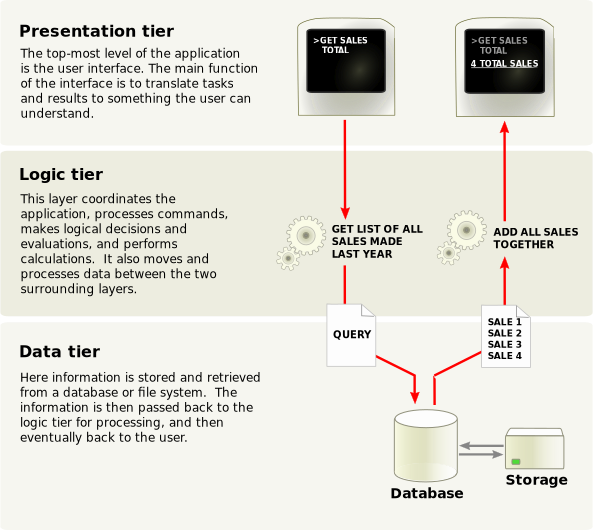
\includegraphics[width=10cm]{threetier}
	\item \textbf{MVC}
	      \begin{itemize}
		      \item Steht für \textit{Model-View-Controller}
		      \item Ziel: Flexibler Programmentwurf; offen für spätere Erweiterungen und Änderungen; Wiederverwendbarkeit einzelner Komponenten
		      \item Besitzt viele Abwandlungen
		      \item Aufbau
		            \begin{itemize}
			            \item Model: enthält Daten, die von der View dargestellt werden; benachrichtigt die View über Änderungen; unabhängig von View und Controller
			            \item View: Darstellung aller GUI-Elemente; unabhängig von Controller; Bekanntgabe an Controller mittels Listener; aktualisiert UI mittels Listener zu Controller
			            \item Controller: Verwaltet View und Model; bekommt UI-Interaktionen von View über Listener; \enquote{schickt} UI-Änderungen an Listener der View; \enquote{schickt} Änderungen von Daten an Listener des Models
		            \end{itemize}
		            \includesvg{mvc}
	      \end{itemize}
	\item \textbf{MVVM}
	      \begin{itemize}
		      \item Steht für \textit{Model-View-ViewModel}
		      \item Variante des MVC; nutzt Datenbindungsmechanismen
		      \item Beispiel: C\# mit WPF (Window Presentation Framework) - \textit{Databindings und Interfaces S.83}
		      \item Trennt Darstellung und Logik
		      \item Im Gegensatz zu MVC muss man nicht für alles Controller implementieren => geringerer Implementierungsaufwand => bessere Testbarkeit
		      \item Durch drei einzelne Instanzen besser testbar (keine extra UI-Tests nötig)
		      \item Rollentrennung von UI-Designern und Entwicklern möglich (z.B. in Firmen)
		      \item Aufbau
		            \begin{itemize}
			            \item Model: \textit{Datenzugriffsschicht}; benachricht über Datenänderungen; führt Validierungen von Benutzereingaben durch; enthält gesamte \enquote{Geschäftslogik}; ist als einzelnes Element mit Unit-Tests testbar
			            \item View: Darstellung aller GUI-Elemente; Bindung zu Viewmodel; einfach austauschbar/modifizierbar/erweiterbar ohne alles andere zu zerstören
			            \item ViewModel: UI-Logik (Model der View); verbindet View und Model; tauscht Informationen mit Model aus; stellt der View Eigenschaften und Befehle zur Verfügung welche von der View and Elemente gebunden werden; hat keine Ahnung von Elementen der View
		            \end{itemize}
		            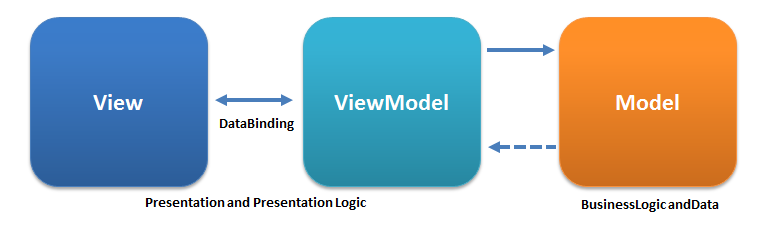
\includegraphics[width=15cm]{mvvm}
	      \end{itemize}
\end{itemize}

\subsection{Projektmanagement}
\begin{itemize}
	\item \textbf{Scrum}
	      \begin{itemize}
		      \item Strikte Rollen: Product Owner (priorisiert Anforderungen), Entwicklungsteam (verantwortlich für die Erreichung der Ziele), Scrum Master (kontrolliert Scrum-Ablauf und Kooperation)
		      \item User Stories: Anforderungen an das Produkt
		      \item Entwicklungsprozess ist in Iterationen (=> \textit{Sprints}) organisiert (brauchen max. 4 Wochen)
		            \begin{enumerate}
			            \item \textbf{Product Backlog}: Team bekommt priorisierte Liste von Anforderungen
			            \item \textbf{Sprint Planning}: Team wählt Teil der Anforderungen als Ziel für diesen Sprint aus (=> nutzbare Zwischen-Version nach Sprint: \textit{Inkrement}); Planung der Zeit, die der Sprint benötigen soll; Organisation: Wer macht was?
			            \item \textbf{Sprint Backlog}: Erstellung des für alle sichtbaren Scrum-Boards (To-Do, In-Progress, Done); Aufteilung der Anforderungen in kleinere Aufgaben (inklusive Tests, Dokumentationen, etc)
			            \item \textbf{Sprint}: Entwickler des Teams arbeiten an ihren jeweiligen Aufgaben
			            \item \textbf{Daily Scrum Meeting}: Max. 15min; täglicher Abgleich des Fortschrittes; Kontrolle und Hilfestellungen einzelner Entwickler; wird wiederholt, bis Sprint zuende ist
			            \item \textbf{Sprint Review}: Am Ende des Sprints; Überprüfung des Inkrements; ggf. Anpassung des Product Backlogs; zurück zum Produkt Backlog wenn alle Anforderungen erfüllt sind
			            \item \textbf{Sprint Retrospektive}: Am Ende des Sprints; Evaluation von Kritik/Verbesserungsvorschlägen am Ablauf
			            \item Zurück zum Sprint Planning für den nächsten Sprint - Sprints werden so lange wiederholt, bis alle Anforderungen erfüllt sind
		            \end{enumerate}
		            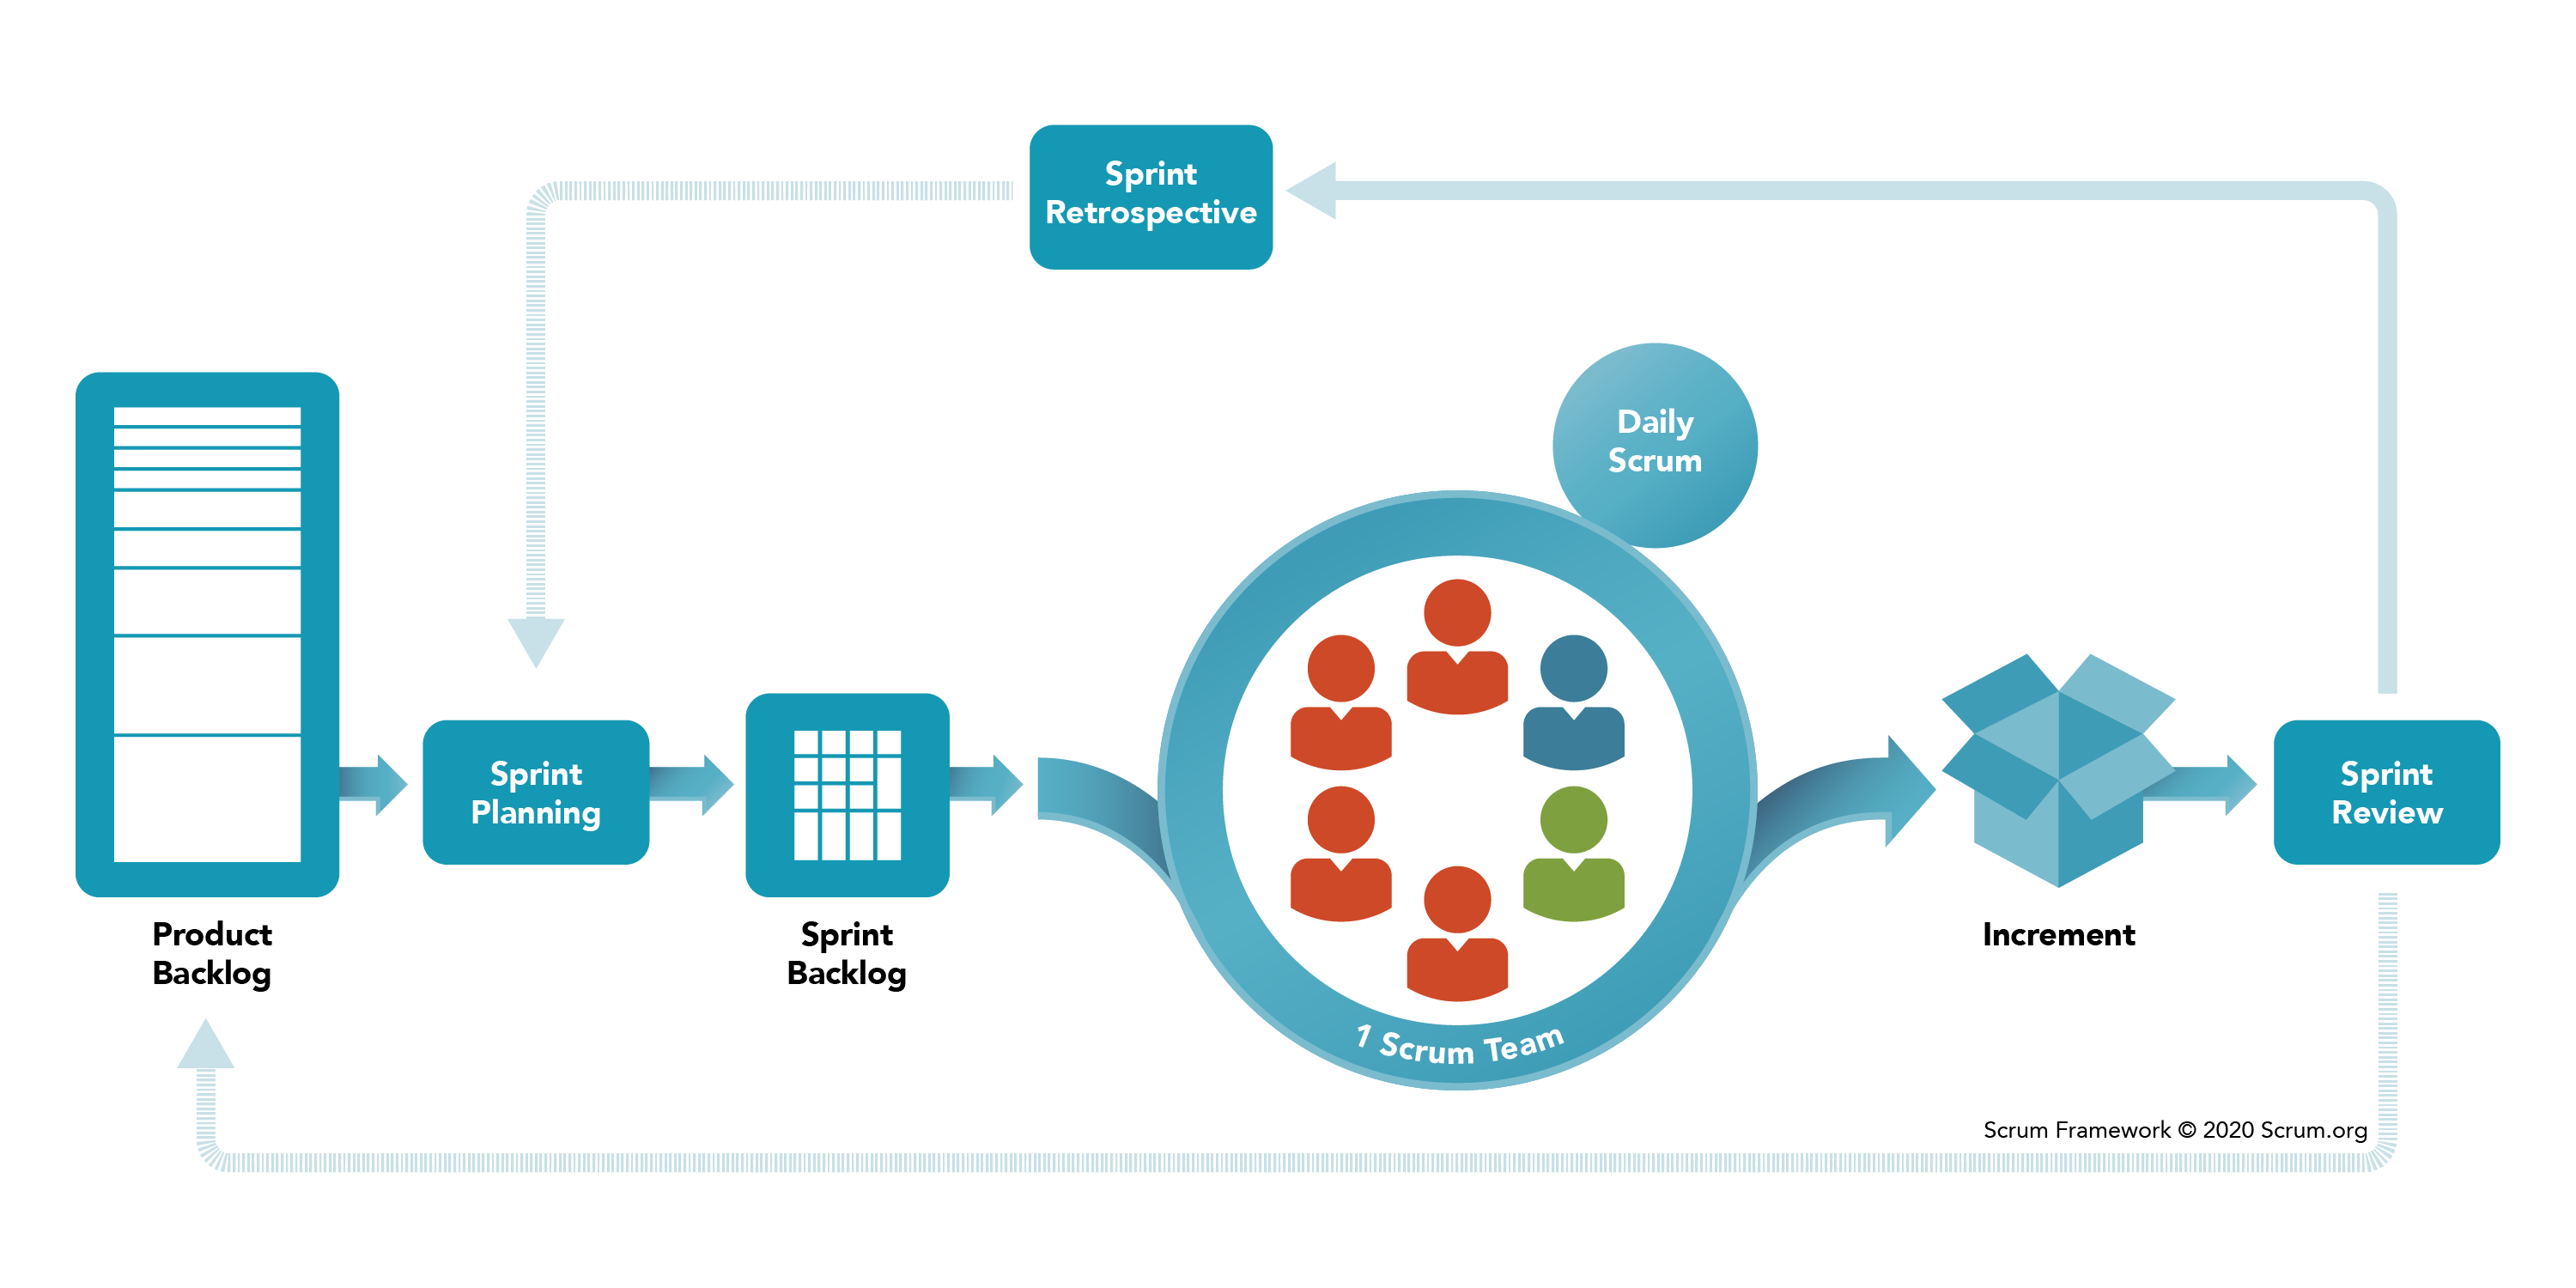
\includegraphics[width=15cm]{scrum}
	      \end{itemize}
	\item \textbf{Wasserfall}
	      \begin{itemize}
		      \item Lineares Modell (im Gegensatz zum iterativen Scrum)
		      \item Sequenziell: Jede Phase muss beendet sein, bevor die nächste anfängt
		      \item Vorteile
		            \begin{itemize}
			            \item Einfach und verständlich
			            \item Klare Abgrenzung der Phasen
			            \item Einfache Möglichkeiten der Planung und Kontrolle
			            \item Bei stabilen Anforderungen: Klare Abschätzung von Kosten und Aufwand
		            \end{itemize}
		      \item Nachteile
		            \begin{itemize}
			            \item Klar abgegrenzte Phasen in der Praxis unrealistisch - häufig fließender Übergang
			            \item In der Praxis sind Rückschritte oft unvermeidlich - in Wasserfall nicht erlaubt
			            \item Unflexibel gegenüber Änderungen
			            \item Frühes Festschreiben der Anforderungen kann problematisch sein, wenn es Änderungen gibt (alles muss erneut durchgeführt werden)
			            \item Kein durchgehendes Testen (wie bei Scrum nach jedem Sprint), sondern erst wenn alles fertig ist (=> potentielle Katastrophe bei finaler Implementation)
		            \end{itemize}
		      \item Typische Phasen
		            \begin{enumerate}
			            \item Anforderungsanalyse (=> Lastenheft)
			            \item Systemdesign (=> Softwarearchitektur)
			            \item Programmierung/Unit-Tests (=> Software)
			            \item Integrations-/Systemtests
			            \item Auslieferung, Einsatz und Wartung
		            \end{enumerate}
	      \end{itemize}
	\item \textbf{Test-Driven-Development} (TDD)
	      \begin{itemize}
		      \item Phasen bei Implementation neuer Features
		            \begin{enumerate}
			            \item Test schreiben, welcher die Spezifikation des Features voll erfüllt
			            \item Alle Tests durchlaufen lassen: Neuer Test muss fehlschlagen (Prävention eines fehlerhaften Tests, welcher immer besteht)
			            \item Einfachste Implementation, die den Test bestehen lässt (muss nicht schön sein, soll einzig und allein den Test bestehen lassen)
			            \item Alle Tests durchlaufen lassen: Alle Tests müssen jetzt bestanden sein
			            \item Refactor: Die neue Implementation lesbarer und wartbarer überarbeiten mit durchgehender Test-Kontrolle
			            \item Für jedes neue Feature wiederholen
		            \end{enumerate}
		      \item Vorteile
		            \begin{itemize}
			            \item Spezifikationen werden schon im Vorraus beachtet (=> weniger Fehleranfällig)
			            \item Implementations-Code wird automatisch möglichst klein, da dieser nur geschrieben wird, um die Tests zu bestehen
			            \item Weniger debugging, da mithilfe der Tests und guten VCS genau verfolgt werden kann, was schiefläuft
			            \item Besser wartbar, weil modularisiert und flexibel
		            \end{itemize}
		      \item Nachteile
		            \begin{itemize}
			            \item Vollständige Tests können vernachlässigt werden, weil Unit-Tests ein falsches Gefühl der Sicherheit verursachen können
			            \item Schlecht geschriebene Tests führen zu schwieriger Wartbarkeit und Implementation neuer Features
			            \item Zeitaufwändig da sehr viele Tests geschrieben werden
			            \item Großer Code-Overhead
		            \end{itemize}
		      \item Beispiele
		            \begin{itemize}
			            \item Tic-Tac-Toe: Test zu Korrektheits-Algorithmen (Diagonal, Horizontal, ...)
			            \item Taschenrechner: Tests für einzelne Funktionalitäten (z.B. Addieren, auch Dinge wie Overflows, etc)
		            \end{itemize}
	      \end{itemize}
\end{itemize}

\subsection{Objektorientierte Programmierung}
\begin{itemize}
	\item Klassen sind \textit{Baupläne} (vgl. Haus-Bauplan)
	\item Objekte sind \textit{Instanzen} der Klassen (vgl. fertiges Haus)
	\item \textbf{Sichtbarkeiten}
	      \begin{itemize}
		      \item \textbf{Public (+)}: Jede Klasse/Methode/... kann darauf zugreifen
		      \item \textbf{Private (-)}: Nur dieselbe Klasse hat Zugriff
		      \item \textbf{Protected (\#)}: Dieselbe Klasse und abgeleitete Klassen (mittels Vererbung) haben Zugriff
	      \end{itemize}
	\item \textbf{Erzeugung}
	      \begin{itemize}
		      \item \textbf{Deklaration}: Primitiv \texttt{int a;} - Komplex \texttt{TolleKlasse b;}
		      \item \textbf{Initialisierung}: Primitiv \texttt{a = 42;} - Komplex \texttt{b = new TolleKlasse();}
	      \end{itemize}
	\item \textbf{Generalisierung}: Enthält die Attribute, die alle Entitäten gemeinsam haben (z.B. abstrakte Klasse \texttt{Tier})
	\item \textbf{Spezialisierung}: Enthält nur die speziell zutreffenden Attribute und erbt von generalisierter Klasse (z.B. \texttt{Nashorn : Tier})
	\item \textbf{Konstruktor}: Wird bei Initialisierung der Klasse aufgerufen. Mit \texttt{: base(...)} kann der Konstruktor der Basisklasse (von der geerbt wird) aufgerufen werden
	\item \textbf{Kapselung}: Nutzung der Sichtbarkeiten, um nur bestimmte Daten zugänglich zu machen. Häufig: Alle Attribute private, Zugriff über public getter/setter Methoden
	\item \textbf{Static}
	      \begin{itemize}
		      \item Member: Statische Member (Attribute, Methoden) bleiben in jeder Instanz gleich
		      \item Klasse: Statische Klassen können nicht instanziiert werden (z.B. Console, Math). Alle Member sind ebenfalls static
	      \end{itemize}
	\item \textbf{Virtual}: Virtuelle Methoden haben eine Implementation, welche von abgeleiteten Klassen (Vererbung) mit \texttt{override} überschrieben werden können
	\item \textbf{Abstract}
	      \begin{itemize}
		      \item Klassen: Können nicht instanziiert werden, nur zum Vererben und für Polymorphie (z.B. \texttt{new List<Tier>();} mit \texttt{Tier} als abstrakte Klasse); kann (muss nicht) abstrakte Methoden enthalten
		      \item Methoden: Müssen in einer abstrakten Klasse deklariert sein und haben keine Implementation; muss von abgeleiteten Klassen (Vererbung) mit \texttt{override} implementiert werden.
	      \end{itemize}
	\item \textbf{Interface}
	      \begin{itemize}
		      \item Enthält nur Signaturen, keine Implementationen
		      \item Anwendung häufig ähnlich wie abstrakte Klassen
		      \item Abgeleitete Klassen müssen \textbf{alle} Methoden implementieren (ohne \texttt{override}), die im Interface deklariert sind
		      \item Unterschied zu abstrakten Klassen: Abgeleitete Klassen von abstrakten Klassen müssen nur diejenigen Methoden implementieren (mit \texttt{override}), die in der Basisklasse abstract sind
	      \end{itemize}
	\item \textbf{Polymorphie} (= \enquote{Mehrere Varianten einer Methode})
	      \begin{itemize}
		      \item Overloading: Methoden können überladen werden, indem eine Methode mit gleichem Namen aber unterschiedlicher Signatur geschrieben wird. Beim Aufruf wird dann automatisch diejenige Implementation gewählt, dessen Signatur mit dem Aufruf übereinstimmt
		      \item Overriding: Geschieht z.B. bei abgeleiteten \texttt{abstract} Klassen oder überschriebenen \texttt{virtual} Methoden
		      \item Statisch: Es steht schon bei Compile-Time fest, welche Operation verwendet werden soll (\textbf{Early Binding}) - beispielsweise mit Overloading
		      \item Dynamisch: Es steht erst bei Run-Time fest, welche Operation verwendet werden soll (\textbf{Late Binding}) - beispielsweise mit Overriding
	      \end{itemize}
	\item \textbf{Properties}
	      \begin{itemize}
		      \item \texttt{public Typ TolleProperty \{ get; set; \}}
		      \item \texttt{public Typ TolleProperty \{ get \{ <getter code> \} set \{ <setter code> \}\}}
		      \item <getter code> bzw. <setter code> könnte bspw. auf private Attribute zugreifen
		      \item get/set optional => Zugriff beschränkbar
		      \item Vorteil zu standard getter/setter: Weniger Code, übersichtlicher, einheitlich
	      \end{itemize}
	\item \textbf{Variablen-Swap}
	      \begin{verbatim}
			int a = 42, b = 69;	
			
			// Langweilig (Dreieckstausch)
			int temp = a;
			a = b;
			b = temp;

			// Besser
			(a, b) = (b, a);

			// 10head
			a ^= b ^= a ^= b;

		\end{verbatim}
\end{itemize}

\subsection{Datenbanken}
\begin{itemize}
	\item \textbf{Primärschlüssel} (PS): Eindeutige Identifizierung (z.B. id)
	\item \textbf{Fremdschlüssel} (FS): Zeigt auf einen PS einer anderen Tabelle; verbindet Tabellen
	\item 1. Normalform: Jedes Attribut ist atomar (unteilbar)
	\item 2. Normalform: 1. NF \&\& jedes Attribut muss vom ganzen PS abhängig sein
	\item 3. Normalform: 2. NF \&\& kein Attribut vom Primärschlüssel transitiv abhängig
	\item \textbf{SQL} (Structured Query Language)
	      \begin{itemize}
		      \item Mögliche Abfrage: \texttt{SELECT DISTINCT \{<spalten> (AS) <name>\} FROM <tabelle1> INNER JOIN <tabelle2> ON <tabelle1.PS> = <tabelle2.FS> WHERE <bedingung> AND/OR/NOT <bedingung> LIKE '\%teil\%' GORUP BY <spalte> HAVING <bedingung> ORDER BY <spalte> ASC/DESC}
		      \item \texttt{Funktionen: AVG(), COUNT(), SUM(), MAX(), MIN()}
	      \end{itemize}
	\item Indizierung von Spalten kann Performance-Probleme bei großen Joins beheben
\end{itemize}

\end{document}
